% Literature review, IEEE conference format (IEEEtran). Built from literature_review_body.tex.
\documentclass[conference]{IEEEtran}
\usepackage{cite}
\usepackage{amsmath,amssymb}
\usepackage{graphicx}
\usepackage{booktabs}
\usepackage{url}
\usepackage{tikz}
\usepackage{pgfplots}
\pgfplotsset{compat=1.17}
\usetikzlibrary{positioning,arrows.meta,calc,fit,backgrounds}
\definecolor{cblue}{HTML}{2D5BD7}
\definecolor{corange}{HTML}{D9822B}
\definecolor{cgreen}{HTML}{1E9E6A}
\definecolor{cgrey}{HTML}{5F6B7A}
\usepackage[hidelinks]{hyperref}

% Second row of authors (standard IEEE conference template macro).
\makeatletter
\newcommand{\linebreakand}{%
  \end{@IEEEauthorhalign}
  \hfill\mbox{}\par
  \mbox{}\hfill\begin{@IEEEauthorhalign}
}
\makeatother
    
\begin{document}

\title{Agentic Defense Against AI-Hallucinated Package Poisoning Using Multi-Agent Dependency Verification}

\author{
\IEEEauthorblockN{Chandan Prakash Hegde}
\IEEEauthorblockA{\textit{Dept. of Information Science}\\
\textit{and Engineering}\\
\textit{Dayananda Sagar College}\\
\textit{of Engineering}\\
Bangalore, India\\
chandanhegde505@gmail.com}
\and
\IEEEauthorblockN{Gaargi L}
\IEEEauthorblockA{\textit{Dept. of Information Science}\\
\textit{and Engineering}\\
\textit{Dayananda Sagar College}\\
\textit{of Engineering}\\
Bangalore, India\\
gaargilm10@gmail.com}
\and
\IEEEauthorblockN{Disha T P}
\IEEEauthorblockA{\textit{Dept. of Information Science}\\
\textit{and Engineering}\\
\textit{Dayananda Sagar College}\\
\textit{of Engineering}\\
Bangalore, India\\
dishap1305@gmail.com}
\linebreakand
\IEEEauthorblockN{Chethan Magudilu Shivanna}
\IEEEauthorblockA{\textit{Dept. of Information Science}\\
\textit{and Engineering}\\
\textit{Dayananda Sagar College}\\
\textit{of Engineering}\\
Bangalore, India\\
chethanms479338@gmail.com}
\and
\IEEEauthorblockN{Spoorthi M}
\IEEEauthorblockA{\textit{Assistant Professor}\\
\textit{Dept. of Information Science}\\
\textit{and Engineering}\\
\textit{Dayananda Sagar College}\\
\textit{of Engineering}\\
Bangalore, India\\
spoorthi.nayaka123@gmail.com}
}

\maketitle
\begin{abstract}
Developers now let language models write their code, pick their dependencies and tell them how to fix a package
that a scanner has flagged. Each of these steps can open the door to a software supply-chain attack. In this paper
we survey 36 sources on package hallucination, typosquatting and package confusion, malicious-package detection,
dependency remediation, and the grounding and verification of model output. For each study we summarize what it
measured and what it found, we compare the closest studies on the tasks and label families they cover, and we
identify six research gaps. The picture is clear. Detection is mature, and hallucinated and vulnerable
dependencies are well measured during code generation. The step that comes after detection, the fix a model
recommends, has hardly been examined: no study checks whether that fix is safe across label families, whether its
reasons are backed by evidence, or what an independent verifier adds. Building on these gaps, we propose a
five-agent architecture in which only one agent uses a language model and a separate rule-based agent checks every
recommendation before it reaches the developer, together with a plan for evaluating it.
\end{abstract}

\begin{IEEEkeywords}
Dependency remediation, large language models, literature survey, malicious packages, package hallucination,
software supply chain security, typosquatting, verification.
\end{IEEEkeywords}

% =====================================================================================================
\section{Introduction}
Public registries such as PyPI and npm let anyone publish a package under any unused name. That openness is what
makes them useful, and it is also what attackers rely on. A misspelled name, a name that imitates a popular
project or a name that a language model tends to invent can all reach a developer who installs it without
checking~\cite{ladisa2023,ohm2020}. Language models have opened a new way in. Spracklen et al.\ found that 19.7\%
of the packages recommended by 16 code models did not exist~\cite{spracklen2025}, and Singla et al.\ found that
coding agents picked a known-vulnerable version in 2.46\% of the dependency changes they made~\cite{singla2026}.

Research on these risks has grown up in separate strands. Hallucination studies look at generated code,
typosquatting and malware studies look at detection, and dependency studies look at update tools, and the strands
rarely meet. This survey brings them together around a single question: once a risky dependency has been found,
can a language model be trusted to recommend a safe fix, and can its reasons be checked? We carried out the survey
before building anything, to decide what such a system should do and how it should be judged. Our contributions are a structured survey of 36
sources (Table~\ref{tab:survey}), a comparison of the closest studies (Table~\ref{tab:compare}), six research gaps,
and a proposed system and evaluation plan that address them (Section~\ref{sec:proposed}).

% =====================================================================================================
\section{Survey Method}
\label{sec:method}
We searched arXiv, publisher and proceedings pages and DOI records in November 2026, using terms such as package
hallucination, slopsquatting, typosquatting, package confusion, malicious package detection, dependency update,
remediation, retrieval-augmented generation and verification. A second set of sources came from the authors' own
archive of IEEE and ACM papers on supply-chain security. We included a source if it measures or detects
hallucinated, typosquatted or malicious packages, studies how dependencies are chosen or updated, or evaluates how
well model output is grounded or verified. One vendor report is included and marked as grey literature. We
confirmed the bibliographic record of every source. Where the full text was available (12 sources) we worked from
it, and otherwise from the abstract. All numbers are reported as the sources state them.

% =====================================================================================================
\section{Literature Survey}
\label{sec:survey}

\subsection{Package hallucination in generated code}
Spracklen et al.~\cite{spracklen2025} generated 576{,}000 code samples with 16 models. Open models invented
packages far more often than commercial ones (21.7\% against 5.2\%). The invented names were also predictable: 43\%
of them came back in all ten repeated runs, and only 13.4\% were within two edits of a real name, so most are not
simple typos. Retrieval, self-refinement and fine-tuning lowered the rate but did not remove it. Krishna
et al.~\cite{krishna2025} showed that the rate depends on the model, the language, the model size and the task.
Twist et al.~\cite{twist2026} changed the developer's request instead of the model and found that models went along
with invented library names in up to 99\% of tasks; a tool that checks whether a name exists in the registry helped
only partly. Raj and Sahu~\cite{raj2026} found that about half of the names flagged in local models already existed
as lookalike packages, which an existence check cannot catch. Miranda-Pena et al.~\cite{mirandapena2026} measured
how far a deterministic static analyzer can go: it caught 14--85\% of library hallucinations. Liu
et al.~\cite{liu2026} built a taxonomy in which library knowledge accounts for 25.99\% of code hallucinations, and
Daoud~\cite{daoud2026} reviewed 16 studies and sorted security-related hallucinations into five types. Li and
Gao~\cite{ligao2025} identified eleven supply-chain threats in generated code, and Latendresse
et al.~\cite{latendresse2024} showed that library recommendations bring license and compatibility problems as well.
Finally, the dataset of Öz~\cite{oz2026} provides reviewed labels for nonexistent Python packages.

\subsection{Typosquatting and package confusion}
Vu et al.~\cite{vu2020} studied typosquatting and combosquatting on PyPI, and Taylor et al.~\cite{taylor2020}
proposed a defense against it. Neupane et al.~\cite{neupane2023} described 13 confusion mechanisms drawn from more
than 1{,}200 attacks, and many of them are semantic rather than spelling-based. Truong et al.~\cite{truong2025}
combined string metrics with a classifier and published labeled typosquat pairs. Jiang et al.~\cite{jiang2026} used
package metadata to bring the false-positive rate of confusion detection down from 80\% to 28\%. Taken together,
these studies show that name similarity alone misses many attacks and raises many false alarms.

\subsection{Malicious packages and their detection}
Ohm et al.~\cite{ohm2020} reviewed real supply-chain attacks, and Ladisa et al.~\cite{ladisa2023} organized 107
attack vectors into a taxonomy that treats typosquatting, dependency confusion and package compromise as separate
attacks. Duan et al.~\cite{duan2021} reported 339 new malicious packages, and Guo et al.~\cite{guo2023} found that
more than 72\% of 4{,}669 malicious PyPI files were still available on mirrors long after they had been discovered.
Detection itself is now strong. Amalfi~\cite{sejfia2022} and SpiderScan~\cite{huang2024} add deterministic or
sandboxed checks to cut false positives, and MalPacDetector~\cite{wang2025mal} keeps only the model-proposed
features that recur. Among the detectors built on language models, Zahan et al.~\cite{zahan2025} reached a
precision of 0.99 on npm, LAMPS~\cite{zeshan2026} splits the work across four cooperating agents,
CHASE~\cite{toda2025} pairs agents with deterministic tools and reached a precision of 0.996, and
IntelGuard~\cite{guo2026} retrieves from threat-intelligence reports. Ryan et al.~\cite{ryan2026} looked at
verdicts and explanations separately across 13 models. The verdicts were often accurate, but the indicators the
models gave to justify them were much weaker, and some did not appear in the package at all.

\subsection{Dependency decisions and remediation}
Decan et al.~\cite{decan2018} showed how vulnerabilities spread through the npm dependency network. Dependabot
reduces technical lag, but developers found the information it gives too sparse to trust and asked for more
transparency~\cite{he2023}. Pearce et al.~\cite{pearce2023} found that models repair synthetic vulnerable code
better than real code. Wang et al.~\cite{wang2026} found that many of the library versions chosen by ten models
carry known vulnerabilities, and fewer do when the version constraints are anchored to external data. Singla
et al.~\cite{singla2026} analyzed 117{,}062 dependency changes and judged each one only against the advisories
published before it was made. A vendor report, which is not peer reviewed, states that 27.8\% of the upgrade
versions recommended by a large model did not exist~\cite{sonatype2026}. The tools used in practice, such as
scanners built on OSV~\cite{osv} and Dependabot, are deterministic. They detect risky dependencies or apply
rule-based updates, but they do not evaluate the advice that model assistants give.

\subsection{Grounding and verification of model output}
Retrieval-augmented generation grounds an answer in retrieved documents~\cite{lewis2020}. Gao et
al.~\cite{gao2023} checked whether generated statements are supported by the passages they cite and found that even
the best systems lacked full support about half of the time. Chain-of-verification lets a model check its own
answer~\cite{dhuliawala2024}, but in the package setting self-refinement helped little~\cite{spracklen2025}. The
alternative is a verifier that shares no model with the generator. Its closest precedents check detections or
generated code~\cite{sejfia2022,toda2025,mirandapena2026}, not the fixes a model recommends.

\begin{table*}[t]
\caption{Summary of the key studies}
\label{tab:survey}
\centering
\small
\setlength{\tabcolsep}{3pt}
\begin{tabular}{@{}p{24mm}p{30mm}p{42mm}p{42mm}p{36mm}@{}}
\toprule
Study & Focus & Data and method & Main finding & Limitation for remediation \\
\midrule
Spracklen~\cite{spracklen2025} & Package hallucination & 16 models, 576k samples, names checked against registries & 19.7\% invented; 43\% repeat in all runs & Generation only \\
Twist~\cite{twist2026} & Developer requests & 7 models, 4{,}173 prompts & Invented names accepted in up to 99\% of tasks & Generation only \\
Raj and Sahu~\cite{raj2026} & Local models & Existence check and classifier & About half of flagged names are registered lookalikes & Response is regeneration \\
Miranda-Pena~\cite{mirandapena2026} & Deterministic checking & Static analysis of generated code & Detects 14--85\% of library hallucinations & Checks code, not fixes \\
Neupane~\cite{neupane2023} & Package confusion & More than 1{,}200 attacks & 13 mechanisms, many semantic & Detection only \\
Jiang~\cite{jiang2026} & Confusion detection & Package metadata, several registries & False positives cut from 80\% to 28\% & Detection only \\
Zahan~\cite{zahan2025} & Malware detection & GPT-4 against CodeQL, 5{,}115 npm packages & Precision 0.99 & Detection only \\
Toda (CHASE)~\cite{toda2025} & Malware detection & Multi-agent with tools, 3{,}000 PyPI packages & Precision 0.996, recall 0.984 & Detection only \\
Ryan~\cite{ryan2026} & Verdicts and reasons & 13 models, 4{,}070 PyPI packages & Indicator F1 0.48 against high verdict F1 & Detection only \\
Wang~\cite{wang2026} & Specified versions & 10 models, 1{,}000 tasks & Many vulnerable versions & Vulnerable family only \\
Singla~\cite{singla2026} & Agent dependency changes & 117{,}062 changes, time-aware & 2.46\% introduce a vulnerable version & No checker, no reasons \\
He~\cite{he2023} & Dependabot & GitHub projects & Lowers lag; trust is limited & Rule-based, no model \\
\bottomrule
\end{tabular}
\end{table*}

% =====================================================================================================
\section{Comparative Analysis}
\label{sec:compare}
Table~\ref{tab:compare} compares the studies closest to model-based remediation on five properties. Two of them make
natural starting points for new work: Spracklen et al.~\cite{spracklen2025} for the scale and predictability of
package hallucination, and Singla et al.~\cite{singla2026} for judging decisions against the advisories known at
the time. Three patterns stand out. First, hallucinated and vulnerable dependencies are well measured during code
generation. Second, malicious-package detection is accurate, and multi-agent and tool-assisted designs are already
established. Third, no study evaluates the fix for a dependency that has already been flagged, and only one checks
the reasons a model gives, and then only on the detection side~\cite{ryan2026}.

\begin{table}[t]
\caption{Properties of the closest studies}
\label{tab:compare}
\centering
\small
\setlength{\tabcolsep}{3pt}
\begin{tabular}{@{}lccccc@{}}
\toprule
Study & Fix & Families & Independent & Time- & Reasons \\
 & evaluated & $>$1 & check & aware & checked \\
\midrule
Spracklen~\cite{spracklen2025} & -- & -- & -- & -- & -- \\
Twist~\cite{twist2026} & -- & -- & partly & -- & -- \\
Miranda-Pena~\cite{mirandapena2026} & -- & -- & $\checkmark$ & -- & -- \\
CHASE~\cite{toda2025} & -- & -- & partly & -- & -- \\
Ryan~\cite{ryan2026} & -- & -- & -- & -- & partly \\
Wang~\cite{wang2026} & -- & -- & -- & -- & -- \\
Singla~\cite{singla2026} & partly & -- & -- & $\checkmark$ & -- \\
Sonatype~\cite{sonatype2026} & partly & $\checkmark$ & -- & -- & -- \\
\midrule
Proposed (planned) & $\checkmark$ & $\checkmark$ & $\checkmark$ & $\checkmark$ & $\checkmark$ \\
\bottomrule
\end{tabular}
\end{table}

% =====================================================================================================
\section{Research Gaps}
\label{sec:gaps}
\textbf{G1: Support for the reasons.} No study checks, claim by claim, whether the reasons a model gives for a
dependency fix are actually supported by the evidence it cites.

\textbf{G2: Safety of the recommended target.} Version studies cover vulnerable and nonexistent
targets~\cite{wang2026,singla2026}. No one has measured whether a proposed replacement is itself malicious or a
typosquat, even though that is exactly the attack described in~\cite{spracklen2025,neupane2023}.

\textbf{G3: Effect and cost of a verifier.} Deterministic stages already exist inside
detectors~\cite{sejfia2022,toda2025}, but no study reports what an independent verifier does to the fixes that are
delivered, including the safe answers it wrongly rejects and the coverage it costs.

\textbf{G4: Rules against models.} Rule-based update tools are established practice~\cite{he2023}, and one vendor
report suggests that they can do better than a model~\cite{sonatype2026}. What is missing is a paired comparison on
the same flagged dependencies.

\textbf{G5: Time-aware evaluation.} Only Singla et al.\ judge decisions against the evidence that was available at
the time~\cite{singla2026}; most studies use the registry as it is today.

\textbf{G6: Families kept separate.} Malicious, typosquat, vulnerable and nonexistent packages are distinct attack
vectors~\cite{ladisa2023}, yet no study compares remediation across them on the same footing.

% =====================================================================================================
\section{Proposed System}
\label{sec:proposed}
All six gaps lead to one requirement: a fix proposed by a language model should be checked by something that does
not share the model's weaknesses. We therefore propose an architecture of five agents (Fig.~\ref{fig:proposed}).

\begin{figure}[t]
\centering
\resizebox{0.92\columnwidth}{!}{%
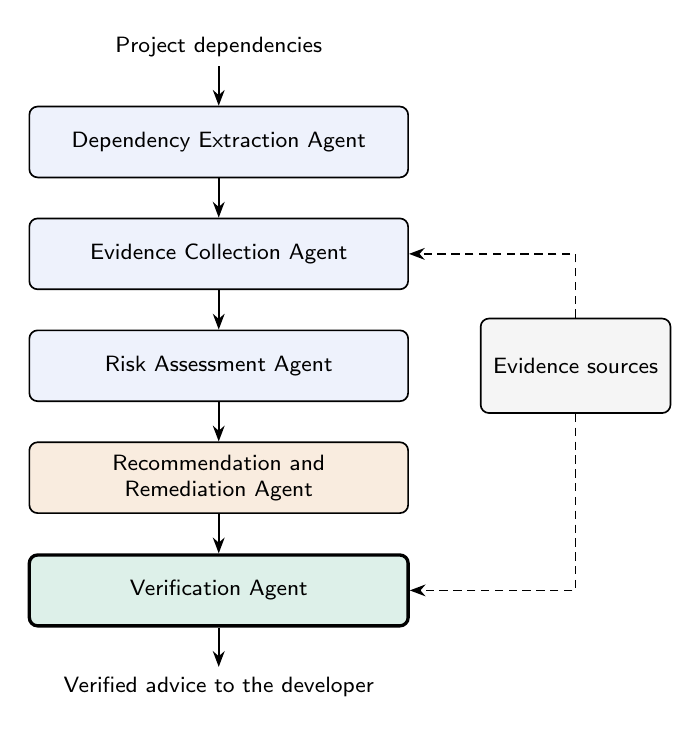
\begin{tikzpicture}[
  font=\sffamily\footnotesize,
  >={Stealth[length=2mm]},
  node distance=5mm,
  agent/.style={draw, rounded corners=3pt, line width=0.6pt, align=center, text width=46mm, minimum height=9mm,
                inner sep=3pt, fill=cblue!8},
  model/.style={agent, fill=corange!15},
  check/.style={agent, fill=cgreen!15, line width=1.2pt},
  side/.style={draw, rounded corners=3pt, line width=0.6pt, align=center, text width=22mm, minimum height=12mm,
               inner sep=3pt, fill=black!4},
  arrow/.style={->, line width=0.7pt},
  read/.style={->, line width=0.6pt, densely dashed}
]
\node[align=center] (in) {Project dependencies};
\node[agent, below=of in] (a1) {Dependency Extraction Agent};
\node[agent, below=of a1] (a2) {Evidence Collection Agent};
\node[agent, below=of a2] (a3) {Risk Assessment Agent};
\node[model, below=of a3] (a4) {Recommendation and Remediation Agent};
\node[check, below=of a4] (a5) {Verification Agent};
\node[align=center, below=of a5] (out) {Verified advice to the developer};
\foreach \x/\y in {in/a1, a1/a2, a2/a3, a3/a4, a4/a5, a5/out} \draw[arrow] (\x) -- (\y);
\node[side, right=9mm of a3] (ev) {Evidence sources};
\draw[read] (ev.north) |- (a2.east);
\draw[read] (ev.south) |- (a5.east);
\end{tikzpicture}}
\caption{Proposed five-agent architecture. Only the Recommendation and Remediation Agent may use a language model;
the Verification Agent checks its output against the evidence.}
\label{fig:proposed}
\end{figure}

The \textbf{Dependency Extraction Agent} will list the project's dependencies. The \textbf{Evidence Collection
Agent} will gather what is known about each package from advisories, malware and typosquat lists, and registry
data. The \textbf{Risk Assessment Agent} will flag risky packages and keep each label family separate. The
\textbf{Recommendation and Remediation Agent} will propose a fix for each flagged package, with reasons that cite
the evidence. It is the only agent allowed to use a language model, and we will also build a rule-based version of
it for comparison. The \textbf{Verification Agent} will check every fix and its reasons against the evidence
before anything reaches the developer. It will share no model with the recommender, and it will hold back any fix
it cannot check.

\textbf{Evaluation plan.} We will evaluate the system on held-out cases from all five label families, running the
recommender with and without the verifier and comparing it with the rule-based recommender. We plan to measure the
share of unsafe fixes, the share of unsupported reasons, coverage (the share of cases that still receive a fix),
and the verifier's precision and recall. To keep hindsight out of the results, part of the evaluation will hide
evidence published after chosen cut-off dates from the system, while the scoring still uses all of it.
Table~\ref{tab:design} shows how the plan answers each gap.

\begin{table}[t]
\caption{How the proposed system addresses each gap}
\label{tab:design}
\centering
\small
\begin{tabular}{@{}p{8mm}p{76mm}@{}}
\toprule
Gap & Planned design choice \\
\midrule
G1 & Reasons must cite evidence; each reason is checked against the record it cites \\
G2 & Every proposed target is checked for being malicious, nonexistent, a typosquat or vulnerable \\
G3 & The same fixes are scored with the verifier off and on, including the coverage lost \\
G4 & A rule-based recommender runs on the same cases as the language model \\
G5 & Cut-off dates hide later evidence from the system but not from the scoring \\
G6 & Each label family is evaluated and reported separately \\
\bottomrule
\end{tabular}
\end{table}

% =====================================================================================================
\section{Challenges and Future Directions}
\label{sec:future}
\textbf{Ground truth.} There is no gold set of correct fixes. Safety can be defined from evidence, but whether a
safe upgrade actually suits a project can only be settled by testing that project. \textbf{Changing evidence.}
Advisories appear after the fact, and mirrors keep malicious files online~\cite{guo2023}, so evaluations need
recorded snapshots and cut-off dates. \textbf{Overlapping sources.} Malicious-package lists copy from each other,
so they are not independent confirmations. \textbf{Explanations.} Verdicts are far more accurate than the
indicators given for them~\cite{ryan2026}, so reasons have to be checked on their own. \textbf{Scale.} Models
change quickly, so results for one set of models may not hold for the next, and any check made when a fix is
chosen cannot see risks that are reported later.

% =====================================================================================================
\section{Conclusion}
Package hallucination and vulnerable version choices are well measured, and malware detection is mature. The step
that turns a detection into a safe outcome, the fix that gets recommended, has received little attention. This
survey identified six gaps around that step. To address them, we proposed a system in which an independent,
rule-based verification stage checks every recommended fix and its reasons against the evidence, together with an
evaluation plan that measures both the safety it adds and the coverage it costs. Building and evaluating this system is the next step
of our work.

% =====================================================================================================
\begin{thebibliography}{99}
% Numbered in order of first citation (IEEE). Page ranges ending in '--' need the
% last page from the publisher record.

\bibitem{ladisa2023}
P.~Ladisa, H.~Plate, M.~Martinez, and O.~Barais,
``Taxonomy of attacks on open-source software supply chains,''
in \emph{Proc. IEEE Symp. Security and Privacy (SP)}, 2023, pp.~1509--1526.

\bibitem{ohm2020}
M.~Ohm, H.~Plate, A.~Sykosch, and M.~Meier,
``Backstabber's knife collection: A review of open source software supply chain attacks,''
in \emph{Proc. DIMVA}, LNCS, 2020, pp.~23--43.

\bibitem{spracklen2025}
J.~Spracklen, R.~Wijewickrama, A.~H.~M.~N.~Sakib, A.~Maiti, B.~Viswanath, and M.~Jadliwala,
``We have a package for you! A comprehensive analysis of package hallucinations by code generating LLMs,''
in \emph{Proc. 34th USENIX Security Symp.}, 2025, pp.~3687--3706.

\bibitem{singla2026}
T.~Singla, B.~{\c{C}}akar, P.~C.~Amusuo, and J.~C.~Davis,
``Towards a benchmark for dependency decision-making,'' arXiv:2601.00205, 2026.

\bibitem{krishna2025}
A.~Krishna, E.~Galinkin, L.~Derczynski, and J.~Martin,
``Importing phantoms: Measuring LLM package hallucination vulnerabilities,'' arXiv:2501.19012, 2025.

\bibitem{twist2026}
L.~Twist, M.~Harman, H.~Yannakoudakis, and J.~M.~Zhang,
``Library hallucinations in LLM-generated code: A risk analysis grounded in developer queries,''
in \emph{Proc. 2026 Conf. Empirical Methods in Natural Language Processing (EMNLP)}, 2026, pp.~1785--1812.

\bibitem{raj2026}
A.~Raj and S.~Sahu,
``Names can hurt: Spotting slopsquatting risks caused by package name hallucinations in local coding LLMs,''
arXiv:2608.23897, 2026.

\bibitem{mirandapena2026}
C.~Miranda-Pena, A.~Reeson, C.~Paris, J.~Poon, and J.~K.~Kummerfeld,
``An empirical analysis of static analysis methods for detection and mitigation of code library
hallucinations,'' \emph{Trans. Machine Learning Research}, 2026, accepted; arXiv:2604.07755.

\bibitem{liu2026}
F.~Liu, Y.~Liu, L.~Shi, Z.~Yang, L.~Zhang, X.~Lian, Z.~Li, and Y.~Ma, ``Beyond functional correctness: Exploring
hallucinations in LLM-generated code,'' \emph{IEEE Trans. Software Engineering}, vol.~52, no.~3, pp.~1037--, 2026.

\bibitem{daoud2026}
S.~Daoud, ``Security-related code hallucinations in large language models: A systematic literature review,'' in
\emph{Proc. Int. Symp. Systems, Advanced Technologies and Knowledge (ISSATK)}, 2026,
doi:10.1109/ISSATK69667.2026.11566869.

\bibitem{ligao2025}
X.~Li and X.~Gao, ``Investigating security implications of automatically generated code on the software supply
chain,'' arXiv:2509.20277, 2025.

\bibitem{latendresse2024}
J.~Latendresse, S.~Khatoonabadi, A.~Abdellatif, and E.~Shihab, ``Is ChatGPT a good software librarian? An
exploratory study on the use of ChatGPT for software library recommendations,'' arXiv:2408.05128, 2024.

\bibitem{oz2026}
E.~S.~Öz, ``Package hallucination in LLM-generated Python code: Data and code,'' Zenodo dataset, v1.0, 2026,
doi:10.5281/zenodo.23962898.

\bibitem{vu2020}
D.-L.~Vu, I.~Pashchenko, F.~Massacci, H.~Plate, and A.~Sabetta,
``Typosquatting and combosquatting attacks on the Python ecosystem,''
in \emph{Proc. IEEE European Symp. Security and Privacy Workshops (EuroS\&PW)}, 2020, pp.~509--514.

\bibitem{taylor2020}
M.~Taylor, R.~Vaidya, D.~Davidson, L.~De~Carli, and V.~Rastogi,
``Defending against package typosquatting,''
in \emph{Network and System Security (NSS)}, LNCS, 2020, pp.~112--131.

\bibitem{neupane2023}
S.~Neupane, G.~Holmes, E.~Wyss, D.~Davidson, and L.~De~Carli,
``Beyond typosquatting: An in-depth look at package confusion,''
in \emph{Proc. 32nd USENIX Security Symp.}, 2023, pp.~3439--3456.

\bibitem{truong2025}
M.~T.~Truong, N.~Gruschka, and L.~Lo~Iacono,
``You can't touch this: Detecting typosquatting packages for enhanced malware prevention in software supply
chains,'' in \emph{Network and System Security (NSS 2024)}, LNCS, Springer, 2025, pp.~147--166.

\bibitem{jiang2026}
W.~Jiang, B.~{\c{C}}akar, M.~Lysenko, and J.~C.~Davis,
``ConfuGuard: Using metadata to detect active and stealthy package confusion attacks accurately and at
scale,'' in \emph{Proc. Int. Conf. Software Engineering (ICSE)}, 2026.

\bibitem{duan2021}
R.~Duan, O.~Alrawi, R.~P.~Kasturi, R.~Elder, B.~Saltaformaggio, and W.~Lee,
``Towards measuring supply chain attacks on package managers for interpreted languages,''
in \emph{Proc. NDSS}, 2021.

\bibitem{guo2023}
W.~Guo, Z.~Xu, C.~Liu, C.~Huang, Y.~Fang, and Y.~Liu,
``An empirical study of malicious code in PyPI ecosystem,''
in \emph{Proc. 38th IEEE/ACM Int. Conf. Automated Software Engineering (ASE)}, 2023.

\bibitem{sejfia2022}
A.~Sejfia and M.~Schäfer, ``Practical automated detection of malicious npm packages,'' in \emph{Proc. 44th
IEEE/ACM Int. Conf. Software Engineering (ICSE)}, 2022, doi:10.1145/3510003.3510104.

\bibitem{huang2024}
Y.~Huang, Z.~Zhou, R.~Wang, S.~Wu, W.~Zheng, S.~Ke, B.~Chen, S.~Gao, and X.~Peng, ``SpiderScan: Practical
detection of malicious NPM packages based on graph-based behavior modeling and matching,'' in \emph{Proc. 39th
IEEE/ACM Int. Conf. Automated Software Engineering (ASE)}, 2024, doi:10.1145/3691620.3695492.

\bibitem{wang2025mal}
J.~Wang, Z.~Li, J.~Qu, D.~Zou, S.~Xu, Z.~Xu, Z.~Wang, and H.~Jin, ``MalPacDetector: An LLM-based malicious NPM
package detector,'' \emph{IEEE Trans. Information Forensics and Security}, vol.~20, pp.~6279--, 2025.

\bibitem{zahan2025}
N.~Zahan, P.~Burckhardt, M.~Lysenko, F.~Aboukhadijeh, and L.~Williams,
``Leveraging large language models to detect npm malicious packages,''
in \emph{Proc. IEEE/ACM 47th Int. Conf. Software Engineering (ICSE)}, 2025, pp.~2625--2637.

\bibitem{zeshan2026}
M.~U.~Zeshan, M.~Ibiyo, C.~Di~Sipio, P.~T.~Nguyen, and D.~Di~Ruscio,
``Many hands make light work: An LLM-based multi-agent system for detecting malicious PyPI packages,''
\emph{J. Systems and Software}, 2026, accepted; arXiv:2601.12148.

\bibitem{toda2025}
T.~Toda and T.~Mori, ``CHASE: LLM agents for dissecting malicious PyPI packages,'' in \emph{Proc. 2nd IEEE/ACM
Int. Conf. AI-powered Software (AIware)}, 2025, doi:10.1109/AIware69974.2025.00008.

\bibitem{guo2026}
W.~Guo, S.~Song, J.~Guo, Z.~Xu, C.~Liu, H.~Ou, M.~Ge, and Y.~Liu, ``Bridging expert reasoning and LLM detection:
A knowledge-driven framework for malicious packages,'' in \emph{Proc. ACM Web Conf.}, 2026, pp.~3554--3565,
doi:10.1145/3774904.3792083.

\bibitem{ryan2026}
A.~Ryan, I.~Khalil, A.~A.~Jahid, M.~Erfan, S.~Park, A.~A.~U.~Rahman, and M.~R.~Rahman,
``An evaluation of large language models for detection of malicious Python packages,'' arXiv:2602.16304, 2026.

\bibitem{decan2018}
A.~Decan, T.~Mens, and E.~Constantinou,
``On the impact of security vulnerabilities in the npm package dependency network,''
in \emph{Proc. 15th Int. Conf. Mining Software Repositories (MSR)}, 2018.

\bibitem{he2023}
R.~He, H.~He, Y.~Zhang, and M.~Zhou,
``Automating dependency updates in practice: An exploratory study on GitHub Dependabot,''
\emph{IEEE Trans. Software Engineering}, 2023.

\bibitem{pearce2023}
H.~Pearce, B.~Tan, B.~Ahmad, R.~Karri, and B.~Dolan-Gavitt,
``Examining zero-shot vulnerability repair with large language models,''
in \emph{Proc. IEEE Symp. Security and Privacy (SP)}, 2023.

\bibitem{wang2026}
Wang, Wu, Ling, Luo, and Zhao,
``Correct code, vulnerable dependencies: A large scale measurement study of LLM-specified library versions,''
arXiv:2605.06279, 2026. % TBD: full author first names

\bibitem{sonatype2026}
Sonatype Inc., ``2026 state of the software supply chain report: AI agents,'' vendor report (not peer
reviewed), 2026. [Online]. Available: \url{https://www.sonatype.com/state-of-the-software-supply-chain/2026/ai-agents}

\bibitem{osv}
Open Source Security Foundation, ``OSV: A distributed vulnerability database for open source,'' [Online].
Available: \url{https://osv.dev}

\bibitem{lewis2020}
P.~Lewis \emph{et al.},
``Retrieval-augmented generation for knowledge-intensive NLP tasks,''
in \emph{Advances in Neural Information Processing Systems (NeurIPS)}, 2020.

\bibitem{gao2023}
T.~Gao, H.~Yen, J.~Yu, and D.~Chen,
``Enabling large language models to generate text with citations,''
in \emph{Proc. EMNLP}, 2023.

\bibitem{dhuliawala2024}
S.~Dhuliawala, M.~Komeili, J.~Xu, R.~Raileanu, X.~Li, A.~Celikyilmaz, and J.~Weston,
``Chain-of-verification reduces hallucination in large language models,''
in \emph{Findings of the Association for Computational Linguistics: ACL 2024}, 2024, pp.~3563--3578.

\end{thebibliography}

\end{document}
